\begin{figure}[t]
  \centering
  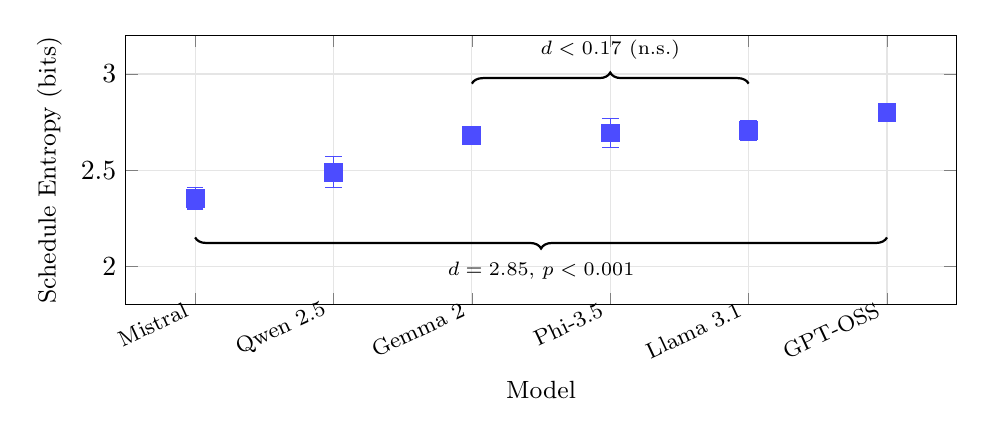
\begin{tikzpicture}
    \begin{axis}[
      width=\columnwidth,
      height=5cm,
      xlabel={Model},
      ylabel={Schedule Entropy (bits)},
      ylabel style={font=\small},
      xlabel style={font=\small},
      symbolic x coords={Mistral, Qwen~2.5, Gemma~2, Phi-3.5, Llama~3.1, GPT-OSS},
      xtick=data,
      x tick label style={font=\footnotesize, rotate=25, anchor=east},
      ymin=1.8, ymax=3.2,
      grid=major,
      grid style={gray!20},
      enlarge x limits=0.1,
      every axis plot/.append style={thick},
    ]
    % Entropy with 95% CI error bars (sorted ascending)
    \addplot[
      only marks, mark=square*, blue!70, mark size=3pt,
      error bars/.cd, y dir=both, y explicit
    ] coordinates {
      (Mistral, 2.354)  +- (0, 0.056)
      (Qwen~2.5, 2.489) +- (0, 0.080)
      (Gemma~2, 2.680)  +- (0, 0.037)
      (Phi-3.5, 2.693)  +- (0, 0.075)
      (Llama~3.1, 2.707)+- (0, 0.053)
      (GPT-OSS, 2.801)  +- (0, 0.032)
    };

    % Significance bracket: middle tier (Gemma, Phi, Llama)
    \draw[decorate, decoration={brace, amplitude=4pt}, thick]
      (axis cs:Gemma~2, 2.95) -- (axis cs:Llama~3.1, 2.95)
      node[midway, above=5pt, font=\scriptsize] {$d<0.17$ (n.s.)};
    \draw[decorate, decoration={brace, amplitude=4pt, mirror}, thick]
      (axis cs:Mistral, 2.15) -- (axis cs:GPT-OSS, 2.15)
      node[midway, below=5pt, font=\scriptsize] {$d=2.85$, $p<0.001$};

    \end{axis}
  \end{tikzpicture}
  \caption{Schedule entropy (diversity) across six LLM models.
  GPT-OSS~20B achieves the highest diversity (2.80~bits);
  Llama~3.1, Phi-3.5, and Gemma~2 form a statistically
  indistinguishable middle tier ($d < 0.17$).
  Mistral~7B produces the least diverse schedules, with a large
  effect size ($d = 2.85$) relative to GPT-OSS.
  Error bars: 95\% CI.}
  \label{fig:ablation-entropy}
\end{figure}
